\documentclass[a4paper, 11pt, spanish]{article}

\usepackage[top=70mm, bottom=30mm, left=18mm, right=18mm]{geometry} % Para modificar el tamaño de las hojas.

\usepackage[spanish]{babel} % Para codificar el texto.

\usepackage{graphicx} % remove the demo option.

\usepackage{fancyhdr} % Para poner la institución, dpto y curso arriba.

\usepackage{amsmath} % Para poder hacer N^o y se vea bonito.

\usepackage[utf8]{inputenc} % Para usar acentos en vez de \'.

\usepackage{parallel} % Para escribir en columnas (Poner los integrantes a la derecha).

\usepackage[firstpage=false]{background} % Para poner el logo de la U arriba en todas las páginas.

% Opciones de background.
\SetBgColor{black}
\SetBgScale{1}
\SetBgOpacity{1}
\SetBgAngle{0}
\SetBgContents{
	\begin{tikzpicture}[remember picture,overlay]
		\node at (-8.0,0.746\textheight) {
\includegraphics[height=18mm,width= 0.155\textwidth]{img/LogoUIngenieria.png}};
	\end{tikzpicture}
}

\fancyheadoffset[L]{-2cm}
\fancyhead[L]{\footnotesize{\textbf{\textsf{Universidad de Chile \\ Facultad de Cs. F\'isicas y Matem\'aticas \\ Departamento de F\'isica \\}}}}
\renewcommand{\headrulewidth}{0pt}
\setlength{\voffset}{-3cm}

\pagestyle{fancy} % Estilo de las páginas

\begin{document}
%\chapter{Algoritmo de Gauss vs Matrices de Rotación}
\vspace*{0.5cm}
\section{Comparacion de la precisión de los algoritmos}
Se estudió el caso de un campo magnético constante en el eje z, $B_0 = 2$, en un intervalo de tiempo fijo $[0, 50]$.

Se estudió la precisión para distintos valores del coeficiente de disipación $\alpha$, tomando valores en [$1$, $0.5$, $0.1$, $0.05$, $0.01$, $0.005$, $0.001$]. Para cada uno de estos valores se estudió la precisión tomando saltos temporales $dt$ en [$5\times 10^{-5}$, $1\times 10^{-4}$, $5\times 10^{-4}$, $1\times 10^{-3}$, $5\times 10^{-3}$, $1\times 10^{-2}$, $5\times 10^{-2}$, $1\times 10^{-1}$, $5\times 10^{-1}$, $1$, $5$].

La precisión se estudió comparando los métodos con la solución analítica, definiendo el error medio por salto de tiempo como:
\begin{equation*}
\varepsilon =  \frac{1}{n} \sum_i |\bar{s}_i- \bar{s}(t_i)|
\end{equation*}\\
En donde $\bar{s}_i$ es el valor obtenido numéricamente y $\bar{s}(t_i)$ es el valor entregado por la solución analítica.
\begin{figure}[!ht]
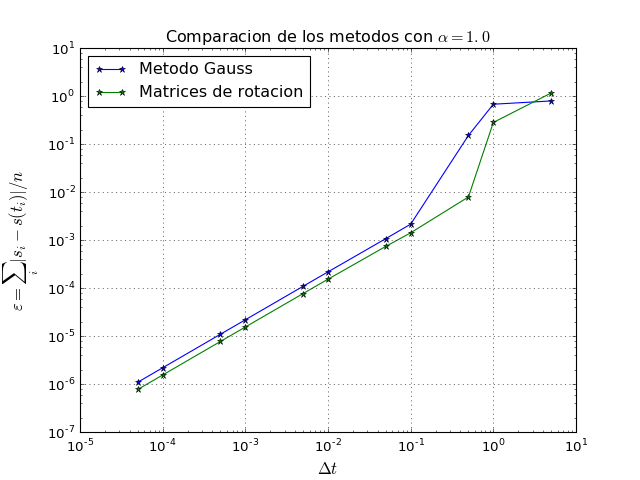
\includegraphics[scale=0.4]{img/comparacion_metodos_1.png}
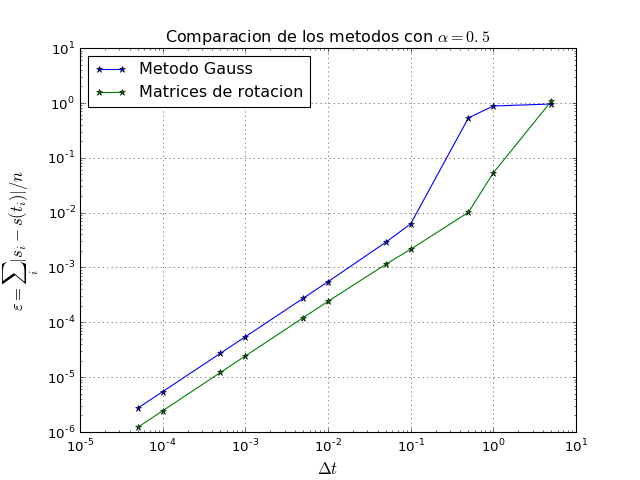
\includegraphics[scale=0.4]{img/comparacion_metodos_5e-1.png}
\end{figure}
\begin{figure}[!ht]
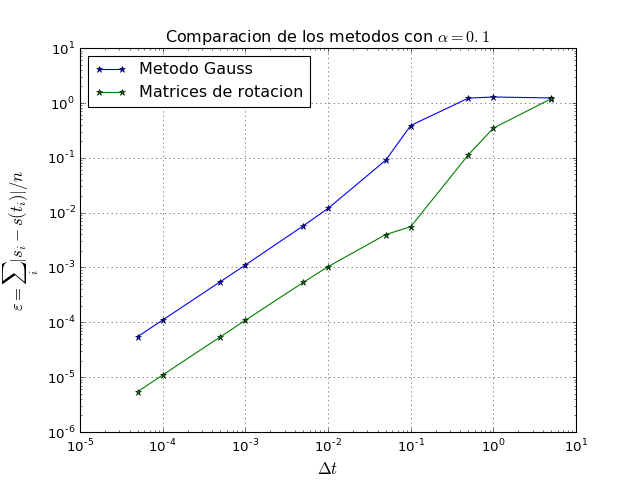
\includegraphics[scale=0.4]{img/comparacio_metodos_1e-1.png}
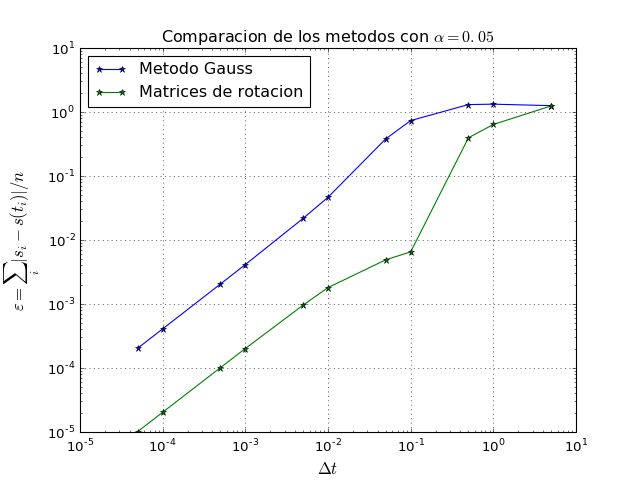
\includegraphics[scale=0.4]{img/comparacion_metodos_5e-2.png}%\end{figure}
\end{figure}
\begin{figure}[!ht]
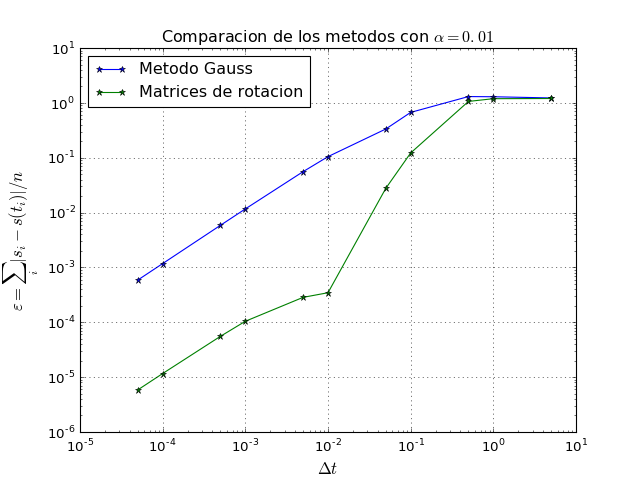
\includegraphics[scale=0.4]{img/comparacion_metodos_1e-2.png}
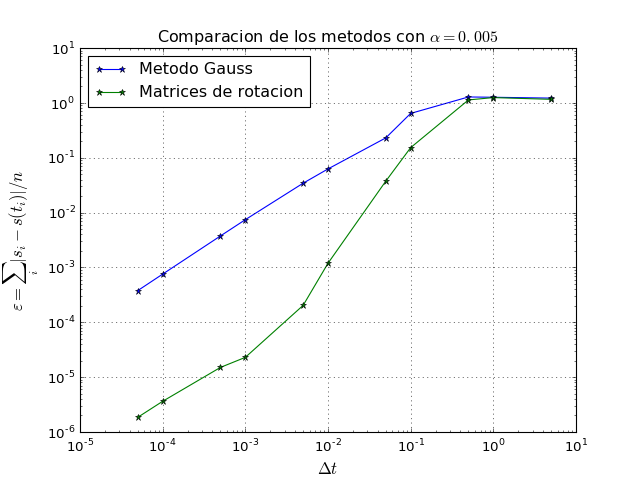
\includegraphics[scale=0.4]{img/comparacion_metodos_5e-3.png}
\end{figure}
\begin{figure}[!ht]
\centering
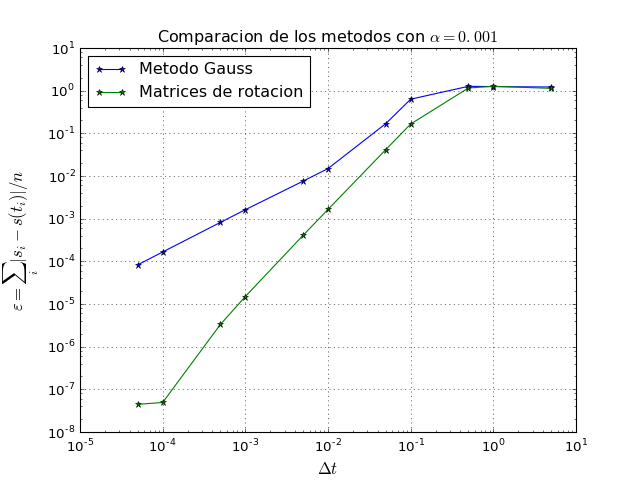
\includegraphics[scale=0.4]{img/comparacion_metodos_1e-3.png}
\end{figure}
\\
\vspace*{15cm}
\section{Comparacion de los tiempos de ejecución}
Se estudio un el mismo campo magnético cte en z, $B_0 = 2$, con coeficiente de disipación $\alpha = 0.05$ en el intervalo temporal $[0,50]$.

\begin{figure}[!ht]
\centering
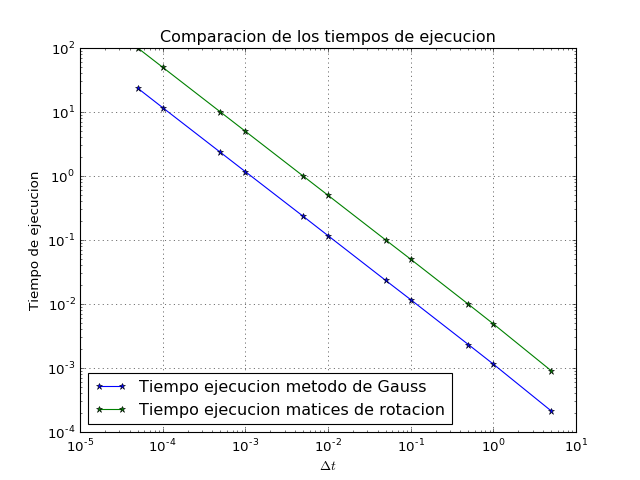
\includegraphics[scale=0.5]{img/comparacion_tiempos_ejecucion.png}
\end{figure}
\newpage
\section{Conclusiones}
En cuanto al error medio por salto de tiempo de los algoritmos, el algoritmo usando matrices de rotación es mucho más preciso, y por tanto puede usarse con saltos de tiempo menos exigentes, obteniendo el mismo orden de error. Ambos se comportan de manera similar para saltos temporales muy grandes, (del orden de dt =1), pero el error es excesivo en ambos así que se descarta inmediatamente este tamaño de saltos `$\Delta t$'.

Como observación, se agrega que los algoritmos funcionan peor a medida que aumentamos el coeficiente de disipación.

En cuanto a los tiempos de ejecución, el algoritmo de las matrices de rotación, casi como regla general, es 4 veces más lento que el algoritmo de Gauss. En particular, tambien se nota que los tiempos de ejecución de ambos algoritmos son de orden $O(n)$ (algoritmos de tiempo lineal), y es por esto que en el gráfico logaritmico se ven como rectas de pendiente -1 ($\Delta t $ aumenta con el inverso de $n$).
\end{document}
